%%%%%%%%%%%%%%%%%%%%%%%%%%%%%%%%%%%%%%%%%%%%%%%%%%%%%%%%%%%%%%%%%%%%%%
% This layout was adapted from one found at latextemplates.com which
% was adapted from another.
%
% License: CC BY-NC-SA 3.0
% (http://creativecommons.org/licenses/by-nc-sa/3.0/)
%
% Original header:
%
% This is a LaTeX version of the sample laboratory report from
% Virginia Tech's copyrighted 08-09 CHEM 1045/1046 lab manual.
% Reproduction of this one appendix section for academic purposes
% should fall under fair use.
%
%%%%%%%%%%%%%%%%%%%%%%%%%%%%%%%%%%%%%%%%%%%%%%%%%%%%%%%%%%%%%%%%%%%%%%

\documentclass{article}

\usepackage{graphicx} % Lets us use images
%\usepackage[acronym]{glossaries} % Lets us use acronyms

\author{Charles Pittman}
\title{ELEC-311\\ Project 2\\ Combinational Circuit Design}
\date{October 1, 2013}

%\loadglsentries{acronyms} % Actually loads 'acronyms.tex'
%\makeglossaries

\begin{document}

\maketitle % Inserts title, author, and date from above

\pagebreak

% Number the enumerate environment (unordered lists) by letter:
\renewcommand{\labelenumi}{\alph{enumi}.}

\section{Objective}
\label{sec:objective}

% Multiple objectives:
 \begin{description}
 \item[First Objective] \hfill \\
   Given a function, design a combinational logic logic circuit.
 \item[Second Objective] \hfill \\
   Minimize the circuit using a Karnaugh map.
 \item[Third Objective] \hfill \\
   Create the circuit using only NAND gates.
 \end{description}

\section{Discussion}
\label{sec:procedure}

The circuit to be constructed was a 2-bit comparator.  A 2-bit
comparator takes two 2-bit numbers, $P = P_1P_0$ and $Q = Q_1Q_0$, and
produces an output, $GT=1 \iff P>Q$.  The truth table describing this
function is shown in Table~\ref{tab:truth}.  This can be displayed
more concisely as a summation of min-terms: $\sum_m(P_1, P_0, Q_1,
Q_0) = (4, 8, 9, 12, 13,14)$.

Using a Karnaugh map (Fig~\ref{fig:k_map}), a minimal form of the
function was found: $GT = P_0 \overline{Q_1 Q_0} + P_1 P_0
\overline{Q_0} + P_1 \overline{Q_1}$.  This function was then
translated into the circuit shown in Fig~\ref{fig:circuit}.

The NAND gate is considered to be a functionally complete set because
any logic function can be created with only NAND gates.  To verify, the
circuit was again translated into one using only NAND gates
(Fig~\ref{fig:circuit_nand}).

\section{Results}
\label{sec:results}

\begin{table}[hbtp]
  \centering
  % This LaTeX table template is generated by emacs 24.3.1
  \begin{tabular}{c|cc|cccc|c}
    $mt$ & $P$ & $Q$ & $P_1$ & $P_0$ & $Q_1$ & $Q_0$ & $GT~(P > Q)$ \\
    \hline
   0 & 0 & 0 & 0 & 0 & 0 & 0 & 0 \\
   1 & 0 & 1 & 0 & 0 & 0 & 1 & 0 \\
   2 & 0 & 2 & 0 & 0 & 1 & 0 & 0 \\
   3 & 0 & 3 & 0 & 0 & 1 & 1 & 0 \\
   4 & 1 & 0 & 0 & 1 & 0 & 0 & 1 \\
   5 & 1 & 1 & 0 & 1 & 0 & 1 & 0 \\
   6 & 1 & 2 & 0 & 1 & 1 & 0 & 0 \\
   7 & 1 & 3 & 0 & 1 & 1 & 1 & 0 \\
   8 & 2 & 0 & 1 & 0 & 0 & 0 & 1 \\
   9 & 2 & 1 & 1 & 0 & 0 & 1 & 1 \\
  10 & 2 & 2 & 1 & 0 & 1 & 0 & 0 \\
  11 & 2 & 3 & 1 & 0 & 1 & 1 & 0 \\
  12 & 3 & 0 & 1 & 1 & 0 & 0 & 1 \\
  13 & 3 & 1 & 1 & 1 & 0 & 1 & 1 \\
  14 & 3 & 2 & 1 & 1 & 1 & 0 & 1 \\
  15 & 3 & 3 & 1 & 1 & 1 & 1 & 0 \\
  \end{tabular}
  \caption{\label{tab:truth}Truth table for 2-bit comparator.}
\end{table}

\begin{figure}[hbtp]
  \centering
  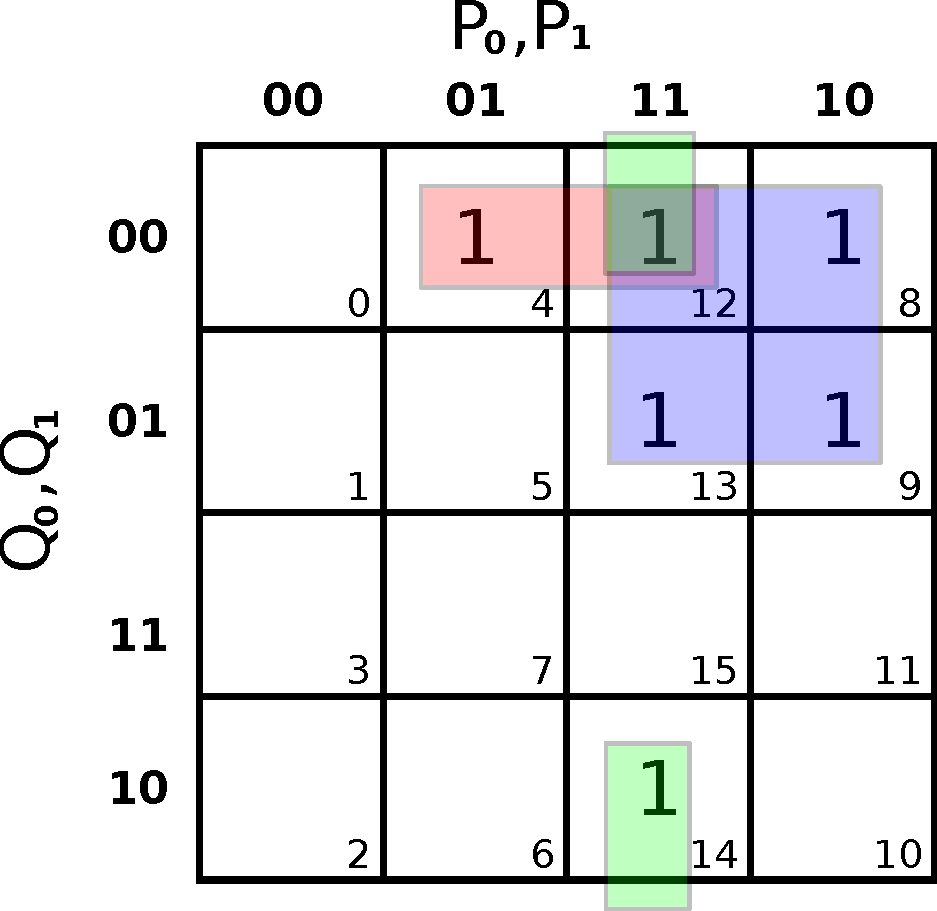
\includegraphics[width=0.5\textwidth]{k_map}
  \caption{\label{fig:k_map} Karnaugh map used to minimize function.}
\end{figure}

\begin{figure}[hbtp]
  \centering
  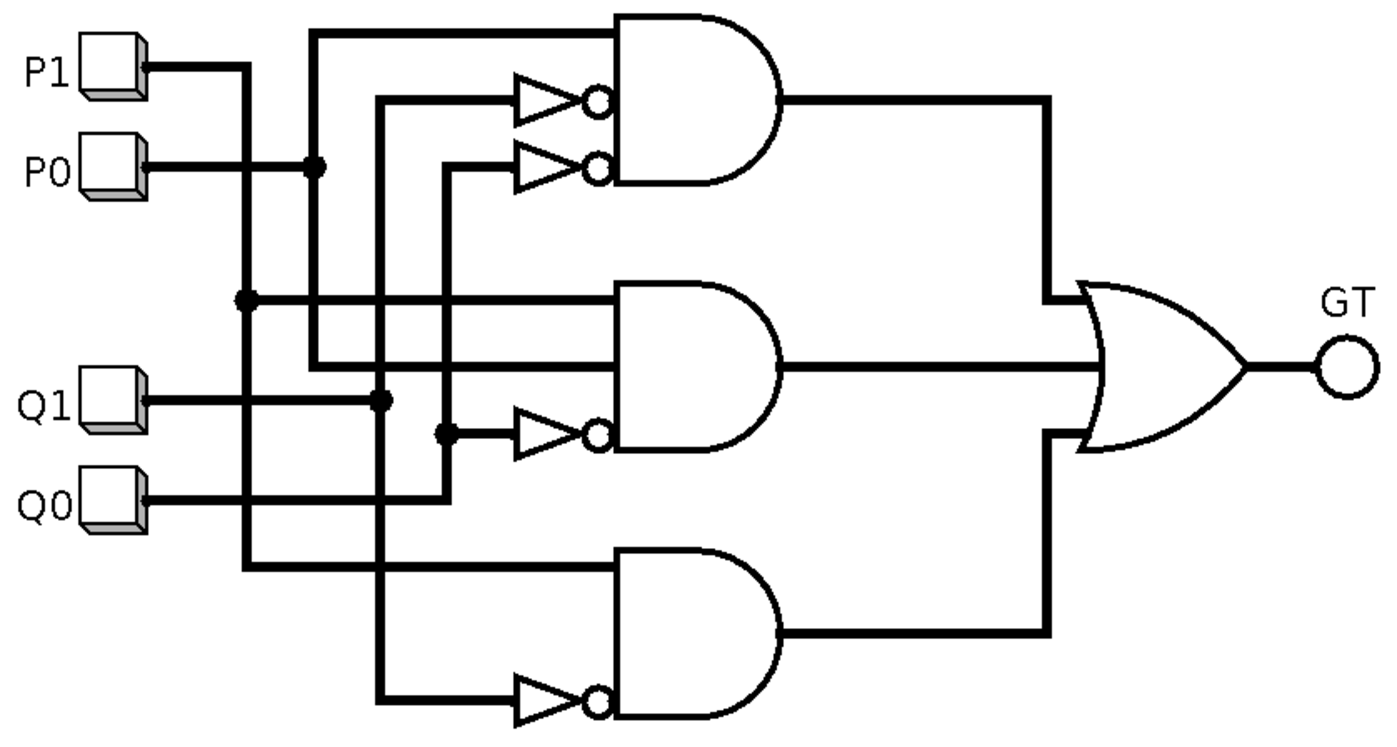
\includegraphics[width=0.8\textwidth]{circuit}
  \caption{\label{fig:circuit} Circuit implemented from function.}
\end{figure}

\begin{figure}[hbtp]
  \centering
  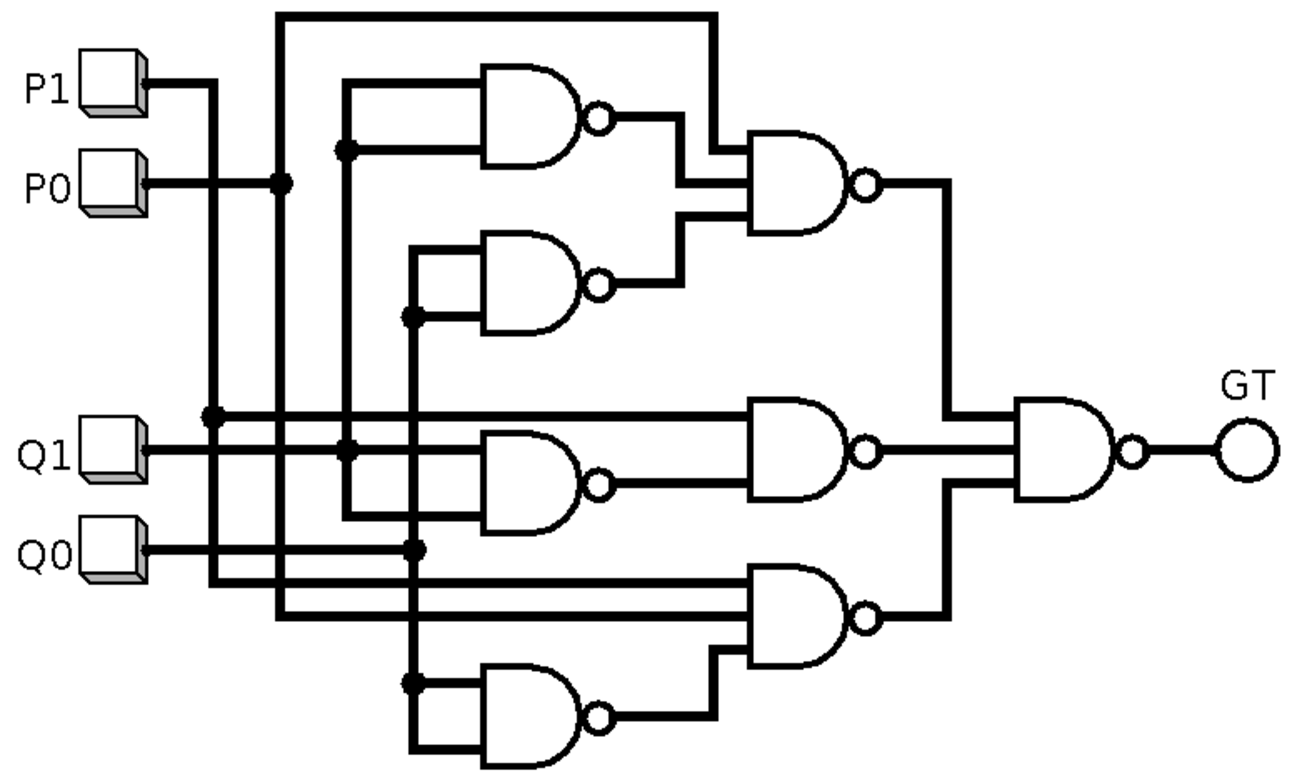
\includegraphics[width=0.8\textwidth]{circuit_nand}
  \caption{\label{fig:circuit_nand} Identical circuit using only NAND gates.}
\end{figure}

\end{document}
